\section{Gas-Filled Detectors} 
%{\color{red} This section still needs to be done!!!}
\subsection{Overview}
\subsubsection{Transportation of Charged Particles in Gases}
\begin{itemize}
    \item Radiation excites and ionizes gases. Per every electron-ion pair created, 30$\sim$35 eV is lost. Without an external electric field, the charges would simply recombine; with the external electric field, particles of opposite charges would drift in opposite directions, resulting in a measurable electric current. 
    \item After the charged particles form, they can undergo various interaction mechanisms with one another or neutral atoms / molecules. The charged particles can participate in random thermal motion and diffuse. During diffusion, the electron may attach to a neutral gas molecule and form a negatively charged ion. Charge transfer motion, where electrons of a neutral molecule are transferred to a positive ion, can also occur; this is especially evident in gas mixtures of various ionization energies. Recombination can also occur when positive ions catch free electrons, or when positive ions and negative ions meet (latter more prominent). 
    \item There are two main types of recombination loss:
    \begin{itemize}
        \item Columnar (initial) recombination:\\
        Ion pairs are formed in a column along the track of the ionizing particle, leading to high local density of ion pairs. This is especially severe for densely ionizing particles such as heavy-charged particles, whose track is shorter in comparison to, say, fast electrons. 
        \item Volume recombination:\\
        Volume recombination occurs when oppositely charged particles meet after they have left their initial position, the aforementioned track. Volume recombination increases with higher irradiation rate, and is therefore combated with higher electric fields. (This feature can be seen in figure~\ref{fig:ion_chamber_saturation_current}.)
    \end{itemize}
    \item An external electric field $E$ ``drifts'' charges to electrodes. The total motion of charges is the superposition of drift and thermal motion.
    \begin{itemize}
        \item The drift velocity is given by $v=\mu E/p$, where $E$ is the electric field strength, $p$ is the gas pressure, and $\mu$ is mobility.
        \item Typical values of $\mu$ fall between $1\sim1.5\times10^{-4}\;m^2s\;atm$\\
        (if $p=1\;atm$ and $E=10^4\;V/m$, then $v\approx1\;m/s$)
        \item Electrons have $\approx1000\times$ higher mobility than ions due to its light mass.
    \end{itemize}
\end{itemize}
\subsubsection{Operational Modes}
\begin{figure}[ht]
    \centering
    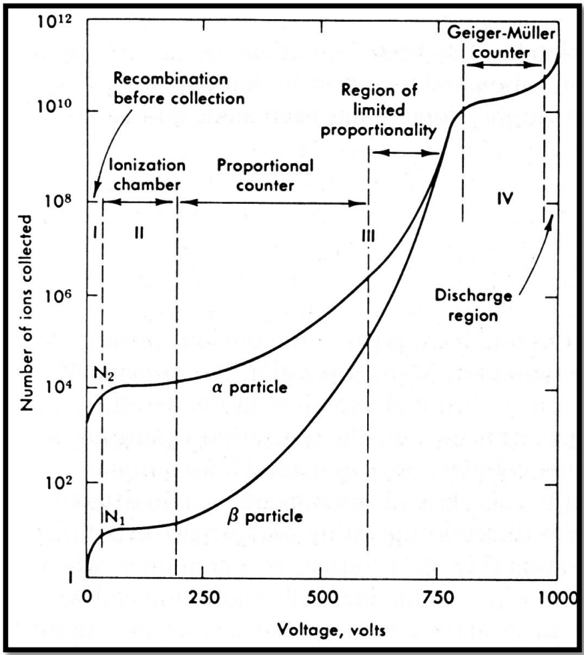
\includegraphics[width=0.5\textwidth]{images/gas_detector_operation_modes.png}
    \caption{Operational modes of gas detectors.}
    \label{fig:gas_detector_operation_modes}
\end{figure}
As shown in figure~\ref{fig:gas_detector_operation_modes}, from low to high voltage, operational modes include (for regions 2, 3, and 5, see following sections for detailed discussions):
\begin{enumerate}
    \item Recombination region (recombination before collection):\\
    Incomplete charge collection
    \item Ionization region (ionization chamber):
    \begin{itemize}
        \item Complete primary charge collection, without multiplication or amplification.
        \item Collected charge is proportional to energy, but signals are small. 
        \item Typically used for heavy charged particle detection or when there are fluxes of radiation.
    \end{itemize}
    \item Proportional counter (proportional counter):
    \begin{itemize}
        \item With electron energies larger than ionization energies, charge multiplication (secondary charge generation) occurs. Signals are amplified by $\approx 10^6$.
        \item Below $\approx600\;V$, the signal amplitude / charge is proportional to energy.
    \end{itemize}
    \item Region of limited proportionality:\\
    Above $\approx600\;V$, due to space charge effects, where positive ions reduce the electric field, there is limited proportionality. 
    \item Geiger-Müller region (GM counter):
    \begin{itemize}
        \item Secondary avalanches occur along the anode wire until the space charge is sufficient to reduce the electric field and suppress multiplication. 
        \item Signals independent of primary charges; no energy information is provided and is only a counter!
    \end{itemize}
    \item Discharge region:
    \begin{itemize}
        \item Continuous discharge occurs with or without radiation present.
        \item To be avoided since this damages the counter.
    \end{itemize}
\end{enumerate}
\subsection{Ionization Chamber}
\subsubsection{Current Mode Operation}
\begin{figure}[ht]
    \centering
    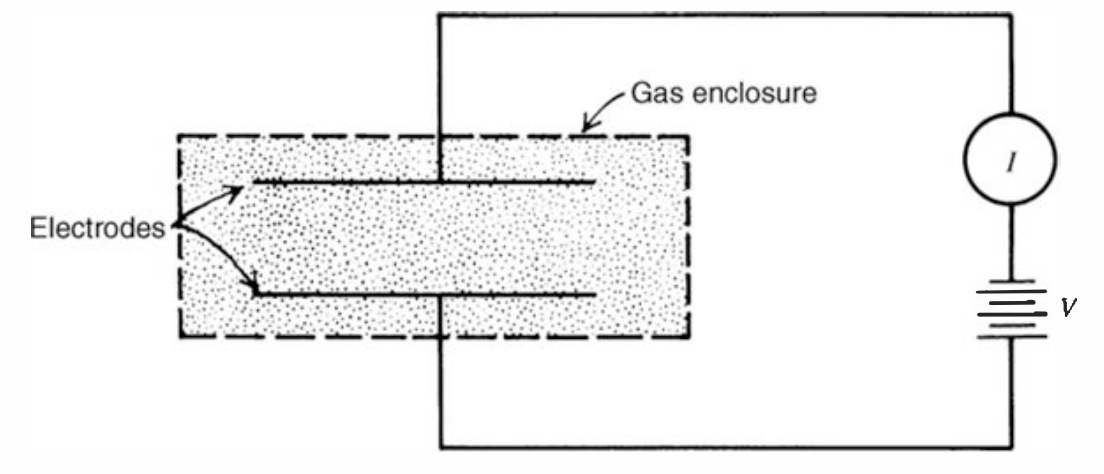
\includegraphics[width=0.5\textwidth]{images/ion_chamber_current_mode.png}
    \caption{Basic elements of an ion chamber.}
    \label{fig:ion_chamber_current_mode}
\end{figure}
\begin{itemize}
    \item The drift of positive and negative charges in an electric field constitutes an electric current. 
    \item As shown in figure~\ref{fig:ion_chamber_current_mode}, the detector is a capacitor with capacity $C$ and stored charge $Q=CV$\\
    The motion of charges in the electric field causes a drop in the stored energy\\ $dE_\text{int}=q_+dV_++q_-dV_-$\\
    which is balanced by the energy supplied by the external circuit\\
    $dE_\text{ext}=VdQ$\\
    $\Rightarrow\;i=\frac{dQ}{dt}=\frac{1}{V}\left(q_+\frac{dV_+}{dt}+q_-\frac{dV_-}{dt}\right)$\\
    With $\frac{dV_\pm}{dt}=\frac{dV_\pm}{dx}\frac{dx}{dt}=E_\pm v_\pm$ and $q_+=q_-=q_0$ , we get $i=\frac{q_0}{V}(v_+E_++v_-E_-)$
    \item The expression found above shows that the signal of an ion chamber is generated by the motion of charges in an electric field, not the arrival of charges at the electrodes.
    \item Assuming constant / steady state irradiation, a constant (saturation) current that reflects the ion pair formation rate will be observed.
    \item As shown in figure~\ref{fig:ion_chamber_saturation_current},as voltage increases, the rate at which the ion pairs are separated increases, and recombination is suppressed. The measured current therefore increases. At a sufficiently high voltage, virtually all recombination is suppressed, and increasing the voltage no longer increases the current since all charges are already collected and their rate of formation is constant. This is the region of ion saturation. 
    \item Due to the aforementioned effects of recombination, higher voltages are needed in the presence of heavy charged particles (columnar recombination) and high irradiation rates (volume recombination). While diffusion of charges will occur due to the existence of a gradient (the concentration of positive ions is greatest near the cathode, and the concentration of negative ions is greatest near the anode), its effects on the saturation current are practically negligible. 
    \item Some additional features of ion chambers include
    \begin{itemize}
        \item sensitivity to energy rate and dose
        \item the use of any fill gases, including those that form negative ions (If recombination is negligible, while the drift velocity of negative ions are thousands of times slower than electrons, they create higher equilibrium concentration of negative charges, and the ion current end up being equal since it is the product of charge density and drift velocity.)
        \item small ion currents and high voltages, resulting in the need of high-quality insulators, guard rings (reduce insulator leakage), and low-noise amplifiers. (1 MeV radiation creates only 0.005 pC of charge)
    \end{itemize}
    \item Ion chambers are used as environmental monitors, survey meters, smoke detectors,  pocket dosimeters, etc., and for measurements of long half-lives, detection of ambient radioactive gases, etc. 
\end{itemize}
\begin{figure}[ht]
    \centering
    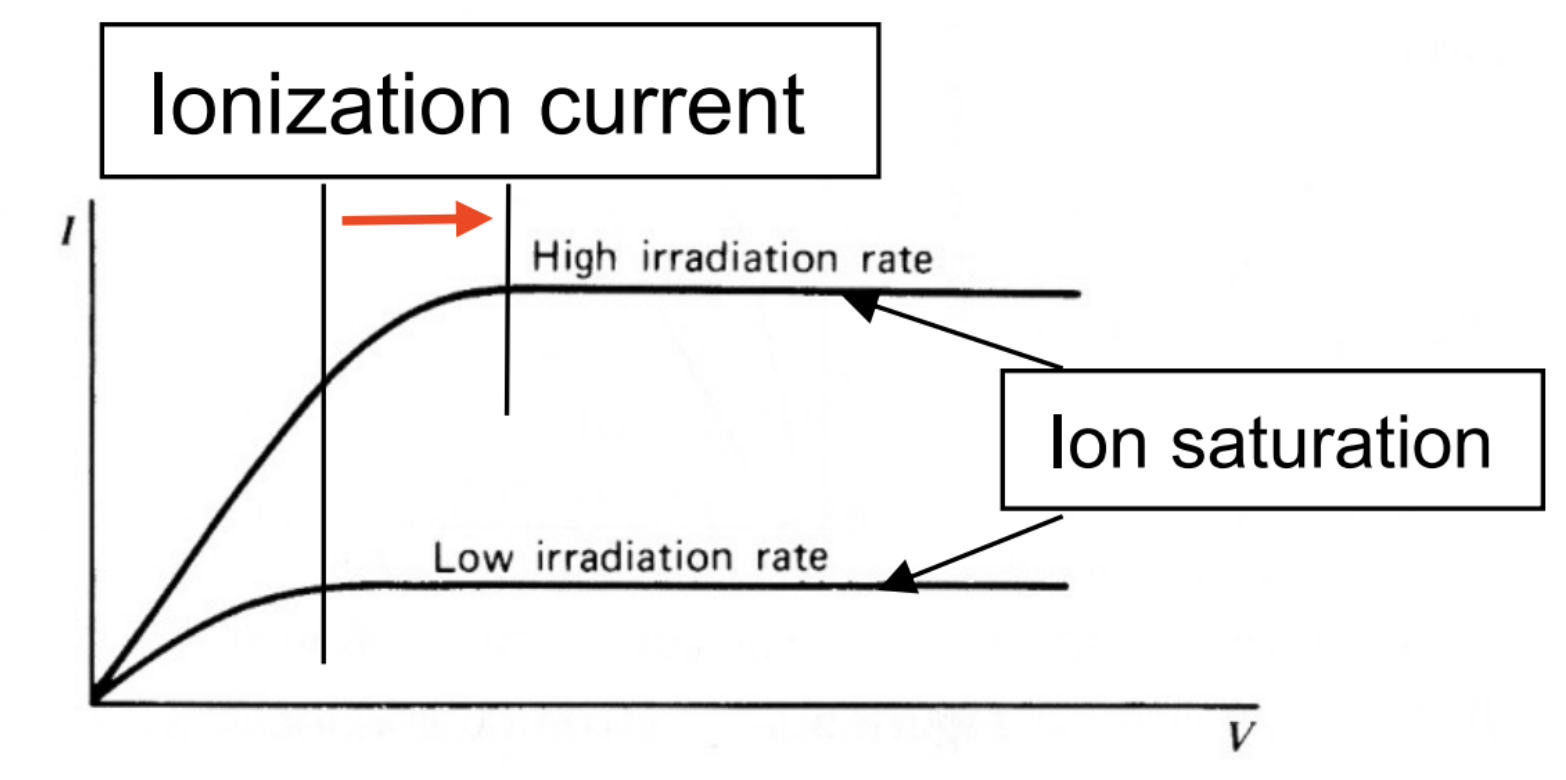
\includegraphics[width=0.5\textwidth]{images/ion_chamber_saturation_current.png}
    \caption{Saturation currents of ion chambers.}
    \label{fig:ion_chamber_saturation_current}
\end{figure}
\subsubsection{Pulse Mode Operation}
{\color{red} This section still needs to be done!!!}

\subsubsection{Energy Resolution and the Fano Factor}
{\color{red} This section still needs to be done!!!}\\
Note that the following calculation methods of energy resolution and the usage of the Fano factor are not exclusive to the context of pulse-mode ionization chambers, but will be applied in future chapters, too.

\subsection{Proportional Counter}
\subsubsection{Operation}
\begin{figure}[ht]
    \centering
    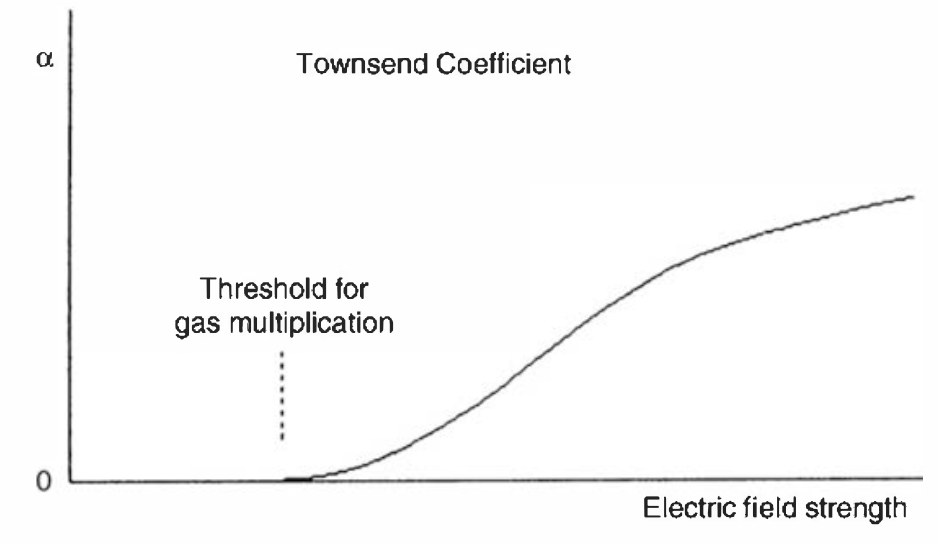
\includegraphics[width=0.5\textwidth]{images/townsend_coefficient.png}
    \caption{Townsend coefficient for gas, $\alpha$.}
    \label{fig:townsend_coefficient}
\end{figure}
\begin{figure}[ht]
    \centering
    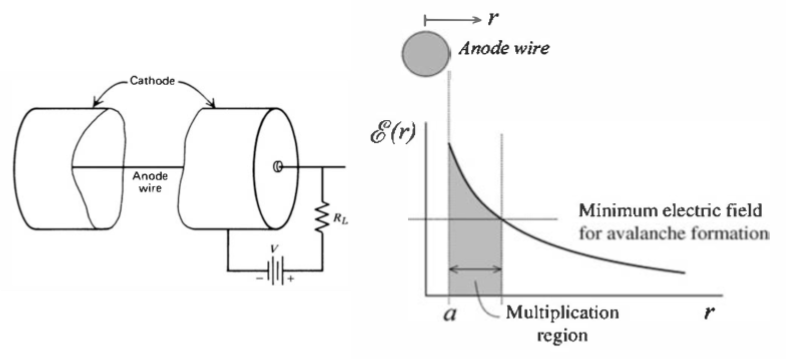
\includegraphics[width=0.6\textwidth]{images/Cylindrical_prop_counter.png}
    \caption{Cylindrical proportional counters geometry and electric field.}
    \label{fig:Cylindrical_prop_counter}
\end{figure}
\begin{itemize}
    \item Proportional counters are usually operated in pulse mode and rely on gas multiplication to amplify charges. Multiplication depends strongly on electric field. 
    \item Townsend avalanches are what allow gas multiplication. Since free electrons are easily accelerated, high electric fields can increase their energy to the degree where they can further ionize neutral molecules during collisions (secondary ionization). The electrons liberated by the secondary ionization process can also be accelerated further and ionize other neutral molecules, leading to a cascade known as a Townsend avalanche. The avalanche terminates when all free electrons are captured at the anode. 
    \item Since each primary electron leads to an independent avalanche, and all avalanches are nearly identical, the collected charges remains proportional to the number of original electrons while the charge is being amplified by thousands of times. 
    \item The fractional increase in the number of electrons per unit path length is governed by the Townsend equation:\\
    $dn/n=\alpha\;dx$, where $\alpha$ is the first Townsend coefficient for gas. As shown in figure~\ref{fig:townsend_coefficient}, $\alpha$ is $0$ when the electric field is below a certain threshold and generally increases when above.\\
    In the case of a spatially constant electric field (e.g. parallel plate), $\alpha$ is constant and $n(x)=n_0e^{\alpha x}$; the density of electrons grows exponentially with distance as the avalanche progresses.
    \item Cylindrical geometries are used in most proportional counters to create high electric fields:\\
    $E(r)={V_0}/[r{\ln(b/a)}]$\\
    ,where $a$ is the anode wire radius and $b$ is the cathode inner radius.\\
    There are two reasons why this geometry is preferred (see figure~\ref{fig:Cylindrical_prop_counter}):
    \begin{itemize}
        \item As can be seen in this expression, the electric field can have a really large value in the vicinity of the anode, to which the electrons are attracted. Using the Townsend equation, since the electric field (and hence $\alpha$) increases in the direction that the avalanche progresses, the growth of electron density is even steeper than in the constant electric field case. The avalanches occur within a few wire diameters of the anode.
        \item To make sure multiplication is uniform, the region of gas multiplication has to be small compared to the total gas volume. With this geometry, the gas multiplication region is confined to the vicinity of the anode. The primary electrons mostly form outside the multiplication region then drift to the multiplication region, ensuring the multiplication factor to be equal for all ion pairs. 
    \end{itemize}
\end{itemize}
\subsubsection{Fill Gas and Quenching}
\begin{itemize}
    \item To avoid the formation negative ions and due to the low working voltage, noble gases are usually used as fill gases for proportional counters. Noble gases can reach up to $10^3$ gain before continuous discharge.
    \item In addition to secondary ionization, molecule excitation can also occur and create photons when the molecule de-excites. These photons reduce proportionality (and space resolution for position-sensitive counters) and are hence not preferred. A quench gas (polyatomic gas) such as methane is used when the gas multiplication is high.  
    \item The most common combination is the P10 gas, a mixture of 90\% Ar and 10\% methane, which can provide gains of up to $10^6$.
\end{itemize}
\subsubsection{Applications}
The proportional counter is used for:
\begin{itemize}
    \item X-ray and electron spectroscopy
    \item Charged particle detection
    \item Discrimination of $\beta$ particles, $\alpha$ particles and fission fragments (superseded by semiconductor detectors)
    \item $2\pi$ and $4\pi$ internal flow counters
    \item Neutron detectors (fill gas $BF_3$ and $^3He$)
    \item Position-sensitive detectors (PPAC, MWPC, TPC,...)
\end{itemize}
\subsection{Geiger-Müller Counter}
\subsubsection{Operation}
\begin{itemize}
    \item Like a proportional counter, a GM counter functions based on gas multiplication. As mentioned in section 6.3.2, free electrons can excite neutral molecules and induce photon production. These photons can undergo photoelectric absorption and create further avalanches. When the electric field is high, the number of excited molecules is much higher than in the proportional region, and Geiger discharge occurs, where an exponentially growing number of avalanches can be created before eventually terminated.
    \item As opposed to a typical Townsend avalanche, in a Geiger discharge, the rapid propagation of the chain reactions leads to avalanche initiations at random radial positions along the wire, as shown in figure~\ref{fig:geiger_discharge}. The Geiger discharge grows to envelope the entire anode wire, regardless of the location of the primary event. 
    \item Geiger discharge is terminated by the buildup of space charges. Since for every free electron produced, a positive ion is produced,  when their concentration is sufficiently high, they can reduce the electric field enough to terminate the multiplication process. 
    \item For a fixed applied voltage, the same density of positive ions is needed to reduce the electric field to below the critical value, no matter what the number of original ion pairs is. The amplitude of the pulses therefore gives no (energy) information of the incident radiation. 
    \item Raising the applied voltage increases the magnitude of the Geiger discharge and the amplitude of the output signal increases (independent of energy deposited). With a fixed discriminator threshold, higher amplitudes imply higher count rates. 
    \item While being inexpensive and easy to use (large signal outputs), Geiger counters provide no energy information and has unusually large dead times ($100\mu s$, very long compared to other detectors). It can be used as a survey meter, or for detection of charged particles when no energy information is needed.
\end{itemize}
\begin{figure}[ht]
    \centering
    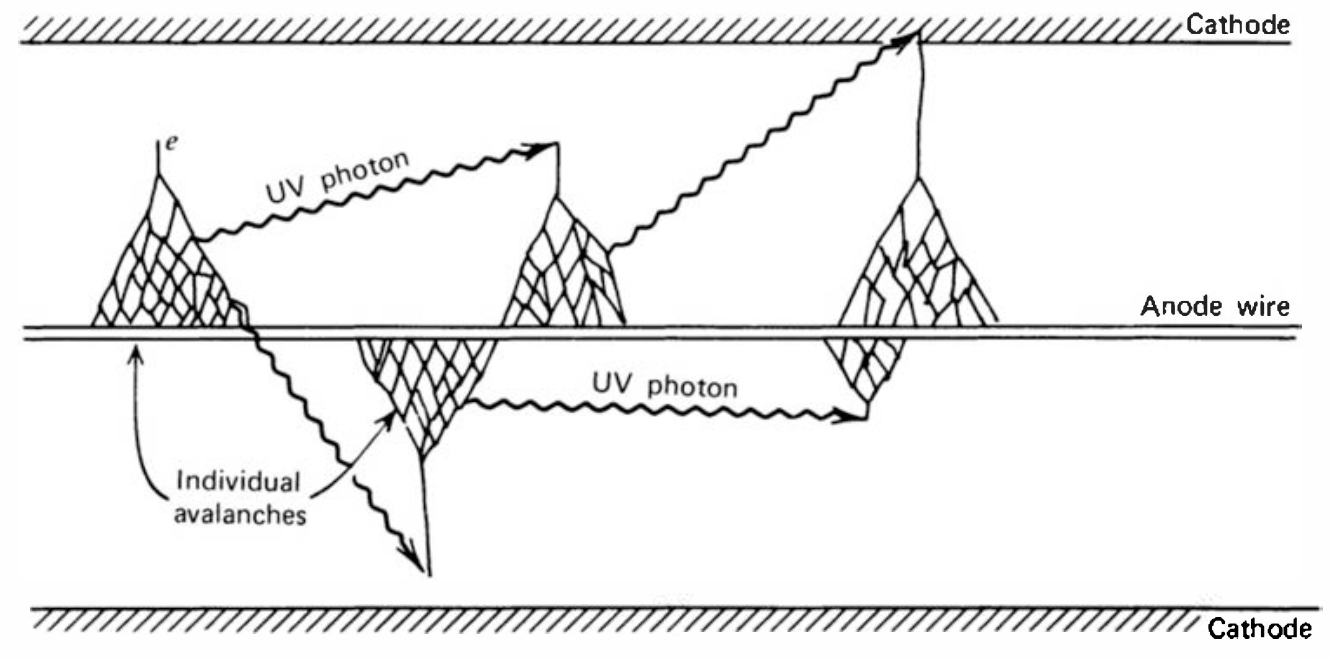
\includegraphics[width=0.5\textwidth]{images/geiger_discharge.png}
    \caption{Geiger discharge.}
    \label{fig:geiger_discharge}
\end{figure}
\subsubsection{Fill Gas and Quenching}
\begin{itemize}
    \item Since GM counters also rely on gas multiplication as in proportional counters, same requirements for fill gases have to be fulfilled; noble gases are usually used. 
    \item Quench gases in GM counters serve a different purpose from those in proportional counters. When a positive ion arrives at the cathode, they are neutralized by combining with an electron from the cathode surface. If the energy liberated in this process exceeds the work function of the cathode, another free electron can emerge. This can lead to multiple pulsing. 
    \item By adding a quench gas of lower ionization energy and a complex molecular structure (e.g., $C_2H_5OHChap$), multiple pulsing can be prevented by the charge transfer collisions between the positive ions with the quench gas. If the concentration of the quench gas is high enough, all the ions that arrive at the cathode will be of the quench gas, and the energy created during their neutralization would go to the dissociation of the complex quench gas molecules instead of the liberation of an electron.  
\end{itemize}

\subsection{Position-Sensitive Detection}